\chapter{Implementierung}

In diesem Kapitel wird die Realisierung der im Konzept beschriebenen Komponenten vorgestellt.
Zu diesem Zweck werden zunächst die dafür verwendeten Rahmenbedingungen wie Systemspezifikation, Entwicklungsumgebung und Software-Versionen definiert.
Im weiteren Verlauf werden die Komponenten und deren mögliche Entwicklung erläutert.

\section{Definition der Entwicklungsumgebung}
Die Software-Komponenten wurden innerhalb einer eigens für diese Arbeit eingerichteten virtuellen Maschine entwickelt, 
da das Visual Studio Projekt des \acs{BCI2000}-Frameworks auf Grund von Kompatibilitätsproblemen ein 32-Bit Betriebssystem erforderte.

\subsubsection{Spezifikation der virtuellen Maschine}
\begin{itemize}
\setlength{\itemsep}{0pt}
%\footnotesize
\item Microsoft Windows 7 Professional SP1 (32-Bit) mit 2 x 3,2 Ghz CPU und 2 GB RAM
\item Microsoft Visual C++ 2010 Express v10.0
\item Adventure Game Studio v3.3.0
\item BCI2000 v3.0.5
\item Qt v4.8.6
\item Cmake v2.8.3
\end{itemize}








\pagebreak
\section{Der \acs{AGS}-P300-Speller}

Das Anwendungsmodul muss gemäß des Konzepts \acs{P300 ERP}'s unterstützen und demzufolge dem "`Oddball-Paradigma"' folgen.
Außerdem muss es die bereits benötigten Parameter Position, Größe und Typ der Speller-Matrix, sowie den aktuellen Bildausschnitt verarbeiten können.\\
Aus diesem Grund wird in den folgenden Unterkapiteln die Entwicklung des "`AGS-P300-Spellers"' nach den oben genannten Rahmenbedingungen, sowie weiterer benötigter Komponenten und Funktionen beschrieben und visualisiert.

\subsection{Speller-Entwicklungsplan}
\vspace{0.3cm}
Die Entwicklung des "`AGS-P300-Speller"' wird auf Basis des bestehenden des P300-Spellers des \acs{BCI}-Systems BCI2000 vorgenommen.
Zu diesem Zweck wird die Revision 4230 des Quellcodes der zuletzt veröffentlichten \acs{BCI2000} Version 3.0.5 (Juli 2012) \cite{Revision4230} verwendet.

Das Erscheinungsbild des P300-Spellers ist in Abbildung \ref{P300SpellerComponents} \textcolor{red}{(1)} zu sehen.\\

\begin{figure}[h!]
\begin{center}
\includegraphics[scale=0.48]{images/P300SpellerBase.png}
\caption{Das Erscheinungsbild des ursprünglichen P300-Spellers (1) mit den dazugehorigen Monitor-Komponenten (2), sowie dem Operator-Modul (3).}
\label{P300SpellerComponents}
\end{center}
\end{figure}







\pagebreak

Die Realisierung erfordert eine Erweiterung des P300-Spellers um Funktionen, welche nachfolgend vereinfacht aufgeführt werden.
\begin{itemize}
\item Die Möglichkeit zur Darstellung des aktuellen Bildausschnitts im Hintergrund
\item Darstellung der Speller-Matrix in variabler Position, Größe und Typ
\item Änderung der Stimulus-Visualisierung von Buchstaben zu halb transparanten Zeilen bzw. Spalten
\item TCI/IP-Kommunikation zwischen Speller und Plugin
\item Durchführung der Stimulus Sequenzen auf Anfrage des Plugins\\
\end{itemize}

Um oben beschriebene Funktionen zu implementieren ist es erforderlich die Architektur des P300-Spellers bzw. des \acs{BCI2000}-Frameworks zu verstehen.\\
Abbildung \ref{ausfuehrungsGraph} zeigt den Ausführungsplan, gemäß der Reihenfolge wie die Ereignisse innerhalb des P300-Spellers auftreten.\\


\begin{figure}[h!]
\begin{center}
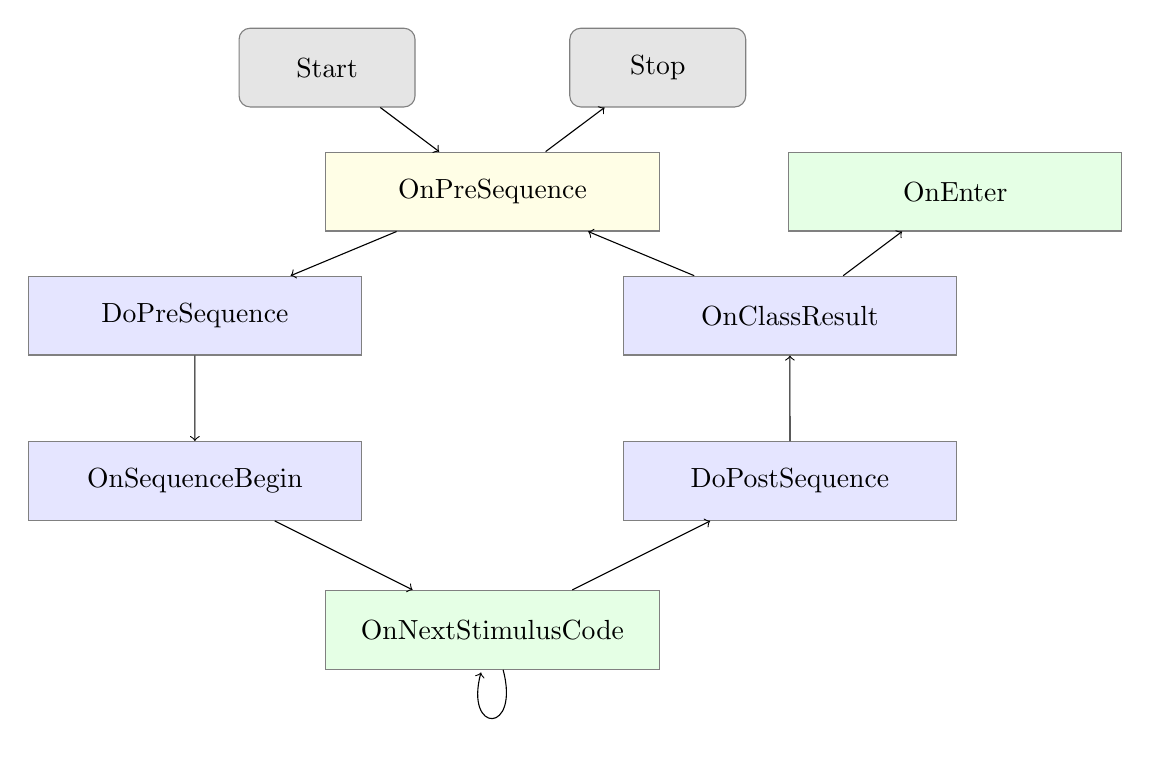
\begin{tikzpicture}[scale=1.05,
rectStart/.style={rectangle, draw=black!50, fill=black!10, minimum width=5mm, minimum height=10mm, text width=20mm, align=center, rounded corners},
rectWait/.style={rectangle, draw=black!50, fill=yellow!10, minimum width=5mm, minimum height=10mm, text width=40mm, align=center},
rectOnce/.style={rectangle, draw=black!50, fill=blue!10, minimum width=5mm, minimum height=10mm, text width=40mm, align=center},
rectLoop/.style={rectangle, draw=black!50, fill=green!10, minimum width=5mm, minimum height=10mm, text width=40mm, align=center},
rectTrigger/.style={rectangle, draw=black!50, fill=green!10, minimum width=5mm, minimum height=10mm, text width=40mm, align=center}
]

% StimulusTask Schleif, insofern sie für uns relevant ist, bzw rein zur Vorstellung

\node[rectStart] (OnStart) at (-2, 4) {Start};
\node[rectStart] (OnStop) at (2, 4) {Stop};
\node[rectWait] (OnPreSequence) at (0, 2.5) {OnPreSequence};
\node[rectOnce] (DoPreSequence) at (-3.598, 1.0) {DoPreSequence};
\node[rectOnce] (OnSequenceBegin) at (-3.598, -1.0) {OnSequenceBegin};
\node[rectLoop] (OnNextStimulusCode) at (0, -2.8) {OnNextStimulusCode}; % loop
\node[rectOnce] (DoPostSequence) at (3.598, -1.0) {DoPostSequence};
\node[rectOnce] (OnClassResult) at (3.598, 1.0) {OnClassResult};
\node[rectTrigger] (OnEnter) at (5.598, 2.5) {OnEnter};



\path[->] 	(OnStart) 				edge 					node {} (OnPreSequence)
			(OnPreSequence) 		edge 					node {} (OnStop)
			(OnClassResult) 		edge 					node {} (OnPreSequence)
			(OnPreSequence) 		edge 					node {} (DoPreSequence)
			(DoPreSequence) 		edge 					node {} (OnSequenceBegin)
			(OnSequenceBegin) 		edge 		 			node {} (OnNextStimulusCode)
			(OnNextStimulusCode) 	edge 		 			node {} (DoPostSequence)
			(DoPostSequence) 		edge 		  			node {} (OnClassResult)
			(OnNextStimulusCode) 	edge 		[loop below]node {} (OnNextStimulusCode)
			(OnClassResult) 		edge 					node {} (OnEnter);
			
\end{tikzpicture}
\caption{Die Ausführungsreihenfolge der internen Funktionen des P300-Spellers}
\label{ausfuehrungsGraph}
\end{center}
\end{figure}



Ausgehend davon das die Konfiguration und Initialisierung innerhalb des Startpunkts abgeschlossen ist, wird mit jedem Schleifen-Durchlauf beginnend bei \textit{OnPreSequence} eine Eingabe ermittelt.
Innerhalb der Schleife werden zunächst die Stimuli erstellt. 
Daraufhin beginnt die Eingabe-Ermittlung indem die Stimuli-Sequenz abgespielt wird, das heißt die Zeilen und Spalten der Speller-Matrix werden angezeigt und wieder ausgeblendet.
Dieser Vorgang entspricht in Abbildung \ref{ausfuehrungsGraph} der Rekursion des \textit{OnNextStimulusCode}-Blocks.
Nach Abschluss der Sequenz wird das resultierende Ergebnis ermittelt und weitergegeben.\\

Innerhalb der nächsten Seiten werden die einzelnen Entwicklungsabschnitte des AGS-P300-Spellers vorgestellt 
und mögliche Szenarien für die Implementierung betrachtet und bewertet. 
Basierend auf dieser Bewertung wird anschließend das zu realisierende Szenario ausgewählt.\\






\pagebreak
\subsection{Darstellung des Hintergrundbilds}
\vspace{0.3cm}

Die Einbindung des Hintergrunds ist ein relativ einfacher, aber sehr wichtiger Aspekt in der Umsetzung des Konzepts, da die Eingabe-Ermittlung außerhalb des Spiels durchgeführt wird.
Der Speller erhält das Bild des aktuellen Spielausschnitts, zeigt dieses im Hintergrund an und überlagert das Bild mit der aktuellen Speller-Matrix. 
Für diesen Zweck muss der Speller erweitert werden, da dieser über keine Möglichkeit zur Manipulation des Hintergrunds verfügt, 
da dies ursprünglich nur über die Textstimulus-Objekte erfolgt und unpraktisch für die Darstellung eines einzelnen Bildes ist.
In Abbildung \ref{bgGraph} wird der Vorgang dargestellt und relativ zu Abbildung \ref{ausfuehrungsGraph} eingeordnet.\\


\begin{figure}[h!]
\begin{center}
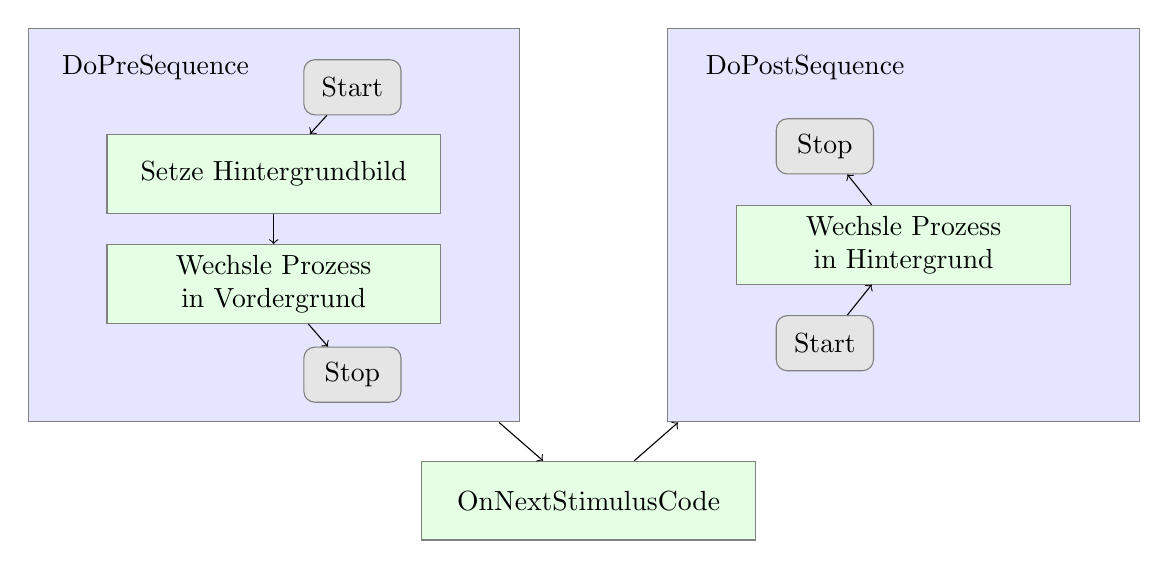
\begin{tikzpicture}[scale=1.0,
rectStartStop/.style={rectangle, draw=black!50, fill=black!10, minimum width=10mm, minimum height=7mm, text width=10mm, align=center, rounded corners},
rectDoPre/.style={rectangle, draw=black!50, fill=blue!10, minimum width=60mm, minimum height=50mm, text width=60mm, align=center},
rectDoPost/.style={rectangle, draw=black!50, fill=blue!10, minimum width=60mm, minimum height=50mm, text width=50mm, align=center},
rectStimulusCode/.style={rectangle, draw=black!50, fill=green!10, minimum width=5mm, minimum height=10mm, text width=40mm, align=center},
rect/.style={rectangle, draw=black!50, fill=green!10, minimum width=5mm, minimum height=10mm, text width=40mm, align=center},
rectVoid/.style={rectangle, draw=black!0, fill=black!0, minimum width=5mm, minimum height=10mm, text width=40mm, align=center}
]

\node[rectDoPre] (DoPreSequence) at (-4, 0) {};
\node[rectDoPost] (DoPostSequence) at (4, 0) {};

\node[rectStimulusCode] (OnNextStimulusCode) at (0, -3.5) {OnNextStimulusCode};


\node at (-5.5, 2) {DoPreSequence};

\node[rectStartStop] (prestart) at (-3, 1.75) {Start};
\node[rect] (image) at (-4, 0.65) {Setze Hintergrundbild};
\node[rect] (foreground) at (-4, -0.75) {Wechsle Prozess in Vordergrund};
\node[rectStartStop] (prestop) at (-3, -1.9) {Stop};



\node at (2.75, 2) {DoPostSequence};

\node[rectStartStop] (poststop) at (3, 1) {Stop};
\node[rect] (background) at (4, -0.25) {Wechsle Prozess in Hintergrund};
\node[rectStartStop] (poststart) at (3, -1.5) {Start};



\path[->] 	(prestart) 					edge 					node {} (image)
			(foreground) 				edge 					node {} (prestop)
			(image) 					edge 					node {} (foreground)
			(poststart) 				edge 					node {} (background)
			(background) 				edge 					node {} (poststop)
			(DoPreSequence) 			edge 					node {} (OnNextStimulusCode)
			(OnNextStimulusCode) 		edge 					node {} (DoPostSequence);



\end{tikzpicture}
\caption{Definition des aktuellen Hintergrunds und Fokussierung auf den Speller}
\label{bgGraph}
\end{center}
\end{figure}

Vor jeder Eingabe-Ermittlung wird das Bild in den Hintergrund des Spellers gesetzt. 
Anschließend ist es vor der Eingabe-Ermittlung erforderlich, dass der Prozess des Spellers in den Vordergrund verschoben wird.
So ersetzt der Speller für den Zeitraum der Eingabe-Ermittlung die Anzeige des Spiels. 
Nach Abschluss dieses Vorgangs wechselt der Speller-Prozess wieder zurück in den Hintergrund.\\





\pagebreak
\subsection{Konfiguration der Speller-Matrix}
\vspace{0.3cm}

Zunächst befassen wir uns mit der Frage, ob es eine Speller-Matrix sein muss oder ob eine andere Variante möglicherweise sinnvoller wäre.
Eine durchaus denkbare Alternative wäre hierfür beispielsweise, dass alle Interaktions-Objekte eines Bildausschnittes jeweils als einzelne Stimuli, 
statt als Zeile oder Spalte aus mehreren Stimuli, gezeigt oder verborgen werden. 
Die Stimuli-Visualisierung kann beispielsweise über das Aufleuchten eines der Objekte erfolgen.
Sofern die Stimuli ebenfalls in zufälliger Reihenfolge dargestellt werden und dem Oddball-Paradigma folgen, spricht auf den ersten Blick nichts gegen eine solche Alternative,
auf den zweiten Blick hingegen ergeben sich einige mögliche Probleme.
Das Oddball-Paradigma erfordert, dass immer eine Mindestmenge verschiedener Stimuli vorhanden ist.
Es entsprechend immer genügend Objekte geben muss oder "`Dummy"'-Objekte hinzugefügt werden müssten.
Weiterhin ist unklar in wie weit sich die Größe einzelner Objekte auf die Ergebnisse auswirken könnte, 
da unterschiedlich große Objekte unterschiedlich viel Aufmerksamkeit auf sich ziehen und entsprechend anders wahrgenommen werden könnten.
Damit wären die Bedinungen des Oddball-Paradigma's verletzt und dieses Szenario nicht mehr anzuwenden.
Sollte allerdings eine einheitliche Größe für alle Objekte gewählt werden können, dann muss zusätzlich gewährleistet werden, dass die Objekte sich nicht überlappen.
Da so \acs{P300 ERP}'s auch bei falschen Objekten ausgelöst werden könnten.\\

Folglich ergibt sich in Anbetracht der beschriebenen Alternative und den möglichen Problemen, dass es offenbar sinnvoll ist den Speller-Matrix-Ansatz weiterhin beizubehalten.\\


Für die Implementierung muss nun die Möglichkeit zur Definition variabler Speller-Matrizzen erarbeitet werden.
Da jede Eingabe-Ermittlung eine eigene Speller-Matrix bedingen kann, 
ist es sinnvoll nach Erhalt der Parameter diese an eine Methode zu übergeben, die die Speller-Matrix aufbaut.

In Abbildung \ref{spellermatrix} ist das Flussdiagramm zu sehen, das die Erstellung einer Speller-Matrix beschreibt.
Die für den Aufbau notwendigen Parameter sind die Position, die Größe und der Typ der Matrix.

\pagebreak 

\begin{figure}[h!]
\begin{center}
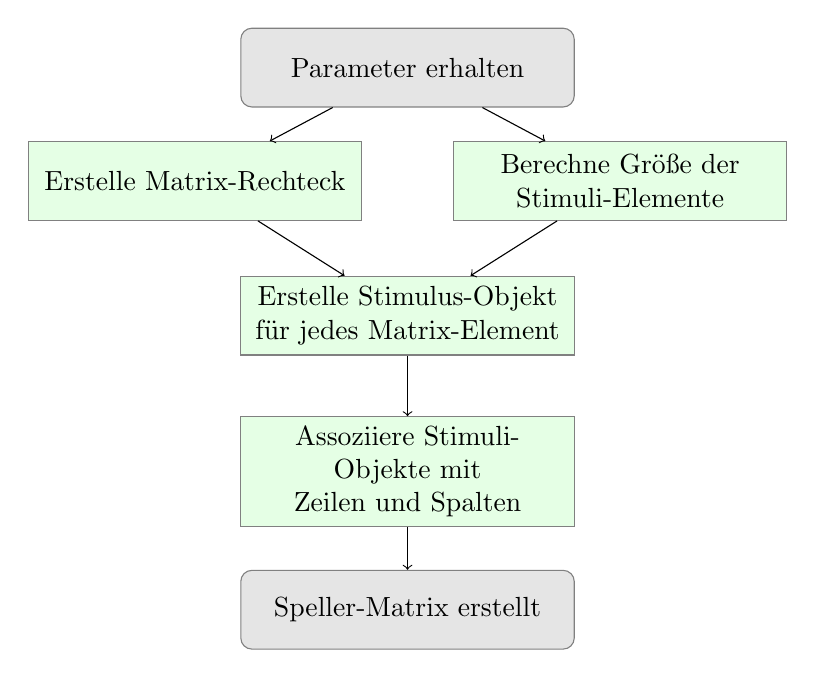
\begin{tikzpicture}[scale=0.9,
rectStart/.style={rectangle, draw=black!50, fill=black!10, minimum width=5mm, minimum height=10mm, text width=40mm, align=center, rounded corners},
rectDoWork/.style={rectangle, draw=black!50, fill=green!10, minimum width=5mm, minimum height=10mm, text width=40mm, align=center},
raute/.style={rectangle,rotate=45,draw=black!100,minimum width=20mm,minimum height=20mm, align=center},
rectText/.style={rectangle, draw=black!0, minimum width=5mm, minimum height=10mm, text width=20mm, align=center}]

\node[rectStart] (Start) at (0, 0) {Parameter erhalten};
\node[rectDoWork] (Matrix) at (-3, -1.6) {Erstelle Matrix-Rechteck};
\node[rectDoWork] (Elements) at (3, -1.6) {Berechne Größe der Stimuli-Elemente};
\node[rectDoWork] (Stimuli) at (0, -3.5) {Erstelle Stimulus-Objekt für jedes Matrix-Element};

%\node[rectText] at (0, -6.25) {Stimuli \\erstellt?};
%\node[raute] (check) at (0, -6.25) {};
%\node at (0.4, -8) {Ja};
%\node at (1.2, -4.9) {Nein};

\node[rectDoWork] (Assoziation) at (0, -5.7) {Assoziiere Stimuli-Objekte mit \\Zeilen und Spalten};
\node[rectStart] (Stop) at (0, -7.65) {Speller-Matrix erstellt};

\path[->] 	(Start) 				edge 					node {} (Matrix)
			(Start) 				edge 					node {} (Elements)
			(Elements) 				edge 					node {} (Stimuli)
			(Matrix) 				edge 					node {} (Stimuli)
			%(Stimuli) 				edge 	[bend right]	node {} (check)
			%(check) 				edge 	[bend right]	node {} (Stimuli)
			%(check) 				edge 					node {} (Assoziation)
			(Stimuli) 				edge 					node {} (Assoziation)
			(Assoziation) 			edge 					node {} (Stop);

\end{tikzpicture}
\caption{Das Flussdiagramm der Speller-Matrix-Erstellung}
\label{spellermatrix}
\end{center}
\end{figure}

Vor jeder neuen Eingabe-Ermittlung werden die damit verbundenen Parameter an die Methode zur Erstellung einer individuellen Speller-Matrix übergeben (zu sehen in Abbildung \ref{matrizzen}).
Anhand der Parameter wird das Rechteck der Speller-Matrix definiert und innerhalb der Anzeige positioniert.
Mit Hilfe des Typs der Matrix wird die Größe jedes Stimulus-Objekts berechnet, sodass über die Zeilen und Spalten iteriert werden kann, um für jedes Element ein Stimulus-Objekt zu erstellen.
Jedes dieser Objekte wird mit seiner entsprechenden Zeile und Spalte in einer Assoziations-Karte verknüpft, 
die für die Assoziation zwischen Stimulus und Signal verantwortlich ist.
Durch diese Verknüpfung kann schließlich das Ergebnis ermittelt werden.

\begin{figure}[ht]
\centering
\includegraphics[scale=0.35]{images/customMatrix.png}
\caption{Eine dynamisch aufgebaute Speller-Matrix des Typs 7x7}
\label{matrizzen}
\end{figure}

Die Erstellung individueller Speller-Matrizen erfüllt weiterhin die Bedingungen des Oddball-Paradigmas, sofern der Typ der Matrix nicht zu klein gewählt wird.


















\pagebreak









\pagebreak
\subsection{Stimulus-Visualisierung}
\vspace{0.3cm}

Gemäß des letzten Kapitels wird weiterhin eine Speller-Matrix verwendet, 
jedoch ist die bisherige Darstellung der Stimuli via aufleuchtender Buchstaben für unsere Bedürfnisse nicht angemessen.
Deshalb ist die Entwicklung eines neuen Stimulus-Derivats erforderlich.
Eine wichtige Anforderung an die neuen Stimuli ist, dass sie einen Reiz unabhängig vom Inhalt erzeugen und somit vor jedem Hintergrundbild dargestellt werden können.\\

Für die Darstellung der Stimuli besteht zum einen die Möglichkeit die Ränder eines Matrix-Elements aufleuchten zu lassen, sodass der Inhalt weiterhin sichtbar ist.
Zum anderen kann die Fläche eines Matrix-Elements halb transparent mit Farbe gefüllt werden, so dass diese Farbe die Fläche überlagert und der Inhalt ebenso sichtbar bleibt.\\

Weiterhin muss jedoch die Anforderung beachtet werden, dass Speller-Matrizen mit beliebiger Position, Größe und Typ dargestellt werden können.
Daraus ergibt sich wie in Abbildung \ref{NoMesh} zu sehen ist, dass es dem Benutzer deutlich erschwert ist sich auf ein Matrix-Element zu fokussieren, wenn dessen Position unbekannt ist.
Eine Eingabe-Ermittlung wird durch diesen Umstand entsprechend erschwert, sodass es sinnvoll ist eine adequate Vorschau zu visualisieren.

\begin{figure}[h!]
\begin{center}
\includegraphics[scale=0.225]{images/NoMesh.png}
\caption{Stimuli-Visualisierung \textbf{ohne} Visualisierung der Speller-Matrix}
\label{NoMesh}
\end{center}
\end{figure}

\pagebreak

Abbildung \ref{Mesh} zeigt die gleiche Szene mit einer Visualisierung der Speller-Matrix.
Die Vorschau ermöglicht es einem Benutzer sich besser auf einen Bereich zu konzentrieren und erlaubt auch vorab den möglichen Eingabebereich besser zu lokalisieren.
Daher erscheint es sinngemäß eine solche Visualisierung auch in der Implementierung zu verwenden, da das Fehlen der Vorschau mit einer Tastatur ohne Tastenbeschriftung gleich käme.\\

\begin{figure}[h!]
\begin{center}
\includegraphics[scale=0.225]{images/Mesh.png}
\caption{Stimuli-Visualisierung \textbf{mit} Visualisierung der Speller-Matrix}
\label{Mesh}
\end{center}
\end{figure}

In Anbetracht der Tatsache, dass in der Implementierung die Matrix durch ein Raster visualisiert wird, 
ist die Darstellung der Stimuli durch aufleuchtende Rahmen möglicherweise nicht in der Lage ausreichend gut wahrgenommen zu werden.
Aus diesem Grund liegt es nahe, die Variante der farbüberlagernden Fläche zu verwenden, wie sie auch schon in den gezeigten Abbildungen verwendet wurde.

\pagebreak
\subsection{Speller-Plugin-Kommunikation}
\vspace{0.3cm}

Die Kommunikation zwischen Speller und Plugin wird ähnlich zu BCI2000 ebenfalls via TCP/IP durchgeführt.
Dabei nimmt der Speller die Rolle eines Servers ein, bei dem sich das Engine Plugin als Client anmelden muss.
In Abbildung \ref{spellerplugintcpip} wird der Ablauf der Kommunikation auf Seiten des Spellers dargestellt.\\

\begin{figure}[h!]
\begin{center}
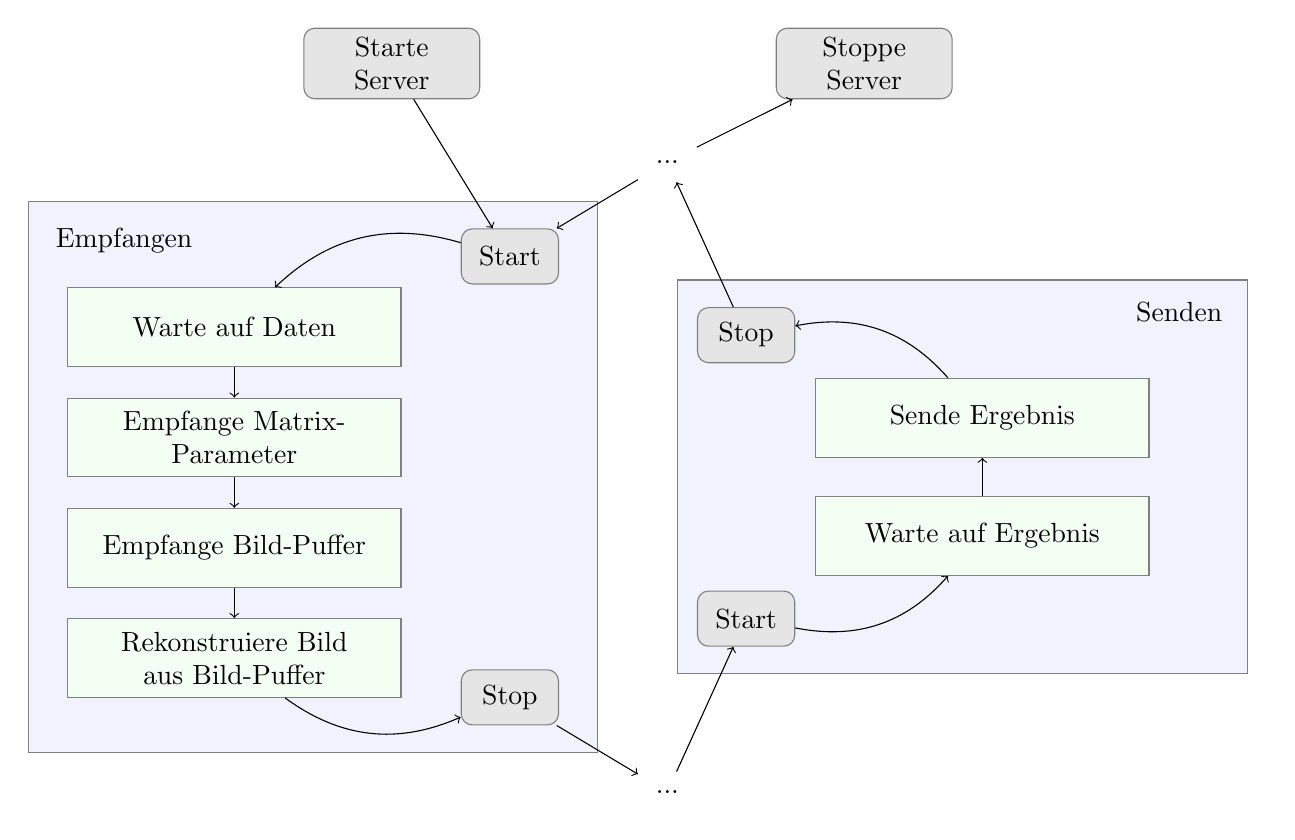
\begin{tikzpicture}[scale=1.0,
rectStart/.style={rectangle, draw=black!50, fill=black!10, minimum width=5mm, minimum height=7mm, text width=10mm, align=center, rounded corners},
rectStart2/.style={rectangle, draw=black!50, fill=black!10, minimum width=5mm, minimum height=7mm, text width=20mm, align=center, rounded corners},
rectDoWork/.style={rectangle, draw=black!50, fill=green!5, minimum width=5mm, minimum height=10mm, text width=40mm, align=center},
rectOnPreSeq/.style={rectangle, draw=black!50, fill=blue!5, minimum width=70mm, minimum height=70mm, text width=70mm, align=center},
rectOnClassRes/.style={rectangle, draw=black!50, fill=blue!5, minimum width=60mm, minimum height=50mm, text width=70mm, align=center},
rectText/.style={minimum width=5mm, minimum height=10mm, text width=20mm, align=center},
rectText2/.style={minimum width=5mm, minimum height=5mm, text width=5mm, align=center}]

\node[rectStart2] (start) at (-3, 5.25) {Starte Server};
\node[rectStart2] (stop) at (3, 5.25) {Stoppe Server};
\node[rectText2] (dots1) at (0.5, 4) {...};
\node[rectText2] (dots2) at (0.5, -4) {...};

% OnPreSequence
\node[rectOnPreSeq] (OnPre) at (-4, 0) {};
\node[rectText] (OnSeqText) at (-6.4, 3) {Empfangen};

\node[rectStart] (OnPreStart) at (-1.5, 2.8) {Start};
\node[rectStart] (OnPreStop) at (-1.5, -2.8) {Stop};

\node[rectDoWork] (waitParams) at (-5, 1.9) {Warte auf Daten};
\node[rectDoWork] (receiveParams) at (-5, 0.5) {Empfange Matrix-Parameter};
\node[rectDoWork] (receiveImage) at (-5, -0.9) {Empfange Bild-Puffer};
\node[rectDoWork] (buildImage) at (-5, -2.3) {Rekonstruiere Bild aus Bild-Puffer};


% OnClassResult
\node[rectOnClassRes] (OnClass) at (4.25, 0) {};
\node[rectText] (OnClassText) at (7, 2.1) {Senden};
\node[rectStart] (OnClassStart) at (1.5, -1.8) {Start};
\node[rectStart] (OnClassStop) at (1.5, 1.8) {Stop};

\node[rectDoWork] (waitResult) at (4.5, -0.75) {Warte auf Ergebnis};
\node[rectDoWork] (sendResult) at (4.5, 0.75) {Sende Ergebnis};


 \path[->] 	 (dots1) 				edge 					node {} (OnPreStart)
			 (OnPreStop) 			edge 					node {} (dots2)
			 (dots2) 				edge 					node {} (OnClassStart)
			 (OnClassStop) 			edge 					node {} (dots1)			
			 (start) 			edge 					node {} (OnPreStart)		
			 (dots1) 			edge 					node {} (stop)				 
			 (OnPreStart) 			edge 		[bend right]node {} (waitParams)
			 (waitParams) 			edge 					node {} (receiveParams)
			 (receiveParams) 		edge 					node {} (receiveImage)		
			 (receiveImage) 		edge 					node {} (buildImage)
			 (buildImage) 			edge 		[bend right]node {} (OnPreStop)
			 (OnClassStart) 		edge 		[bend right]node {} (waitResult)
			 (waitResult) 			edge 					node {} (sendResult)			 
			 (sendResult) 			edge 		[bend right]node {} (OnClassStop);

\end{tikzpicture}
\caption{Die Ausführungsreihenfolge der TCP/IP-Kommunikation auf Seiten des AGS-P300-Spellers}
\label{spellerplugintcpip}
\end{center}
\end{figure}

Bei jeder Anfrage werden zunächst die Parameter der Speller-Matrix übertragen. 
Anschließend werden die Bild-Daten gepuffert und das Bild anhand der Daten rekonstruiert.
Sobald dieser Vorgang abgeschlossen ist werden die Parameter und das Bild weitergegeben, sodass der Speller fortfahren kann.\\

Nach Abschluss und Ermittlung der Eingabe wird das Ergebnis an das Plugin zurückgesendet und dort verarbeitet.
Der Speller wird während dieser Zeit auf eine erneute Anfrage des Spiels warten.









\pagebreak
\section{Das AGS-P300-Plugin}

Dieses Kapitel befasst sich mit der Entwicklung eines Engine Plugins und soll die Schnittstelle zwischen AGS-Spiel und Speller darstellen,
so dass die Kommunikation zwischen Spiel und Speller ermöglicht wird.\\

Aus diesem Grund ist der Funktionsumfang des Plugins im Vergleich zum Speller relativ gering, da lediglich die Daten aufbereitet, versendet und wieder empfangen werden müssen.\\
In Abbildung \ref{pluginPlan} werden die inneren und äußeren Abläufe aus Sicht des Plugins dargestellt.\\




\begin{figure}[h!]
\begin{center}
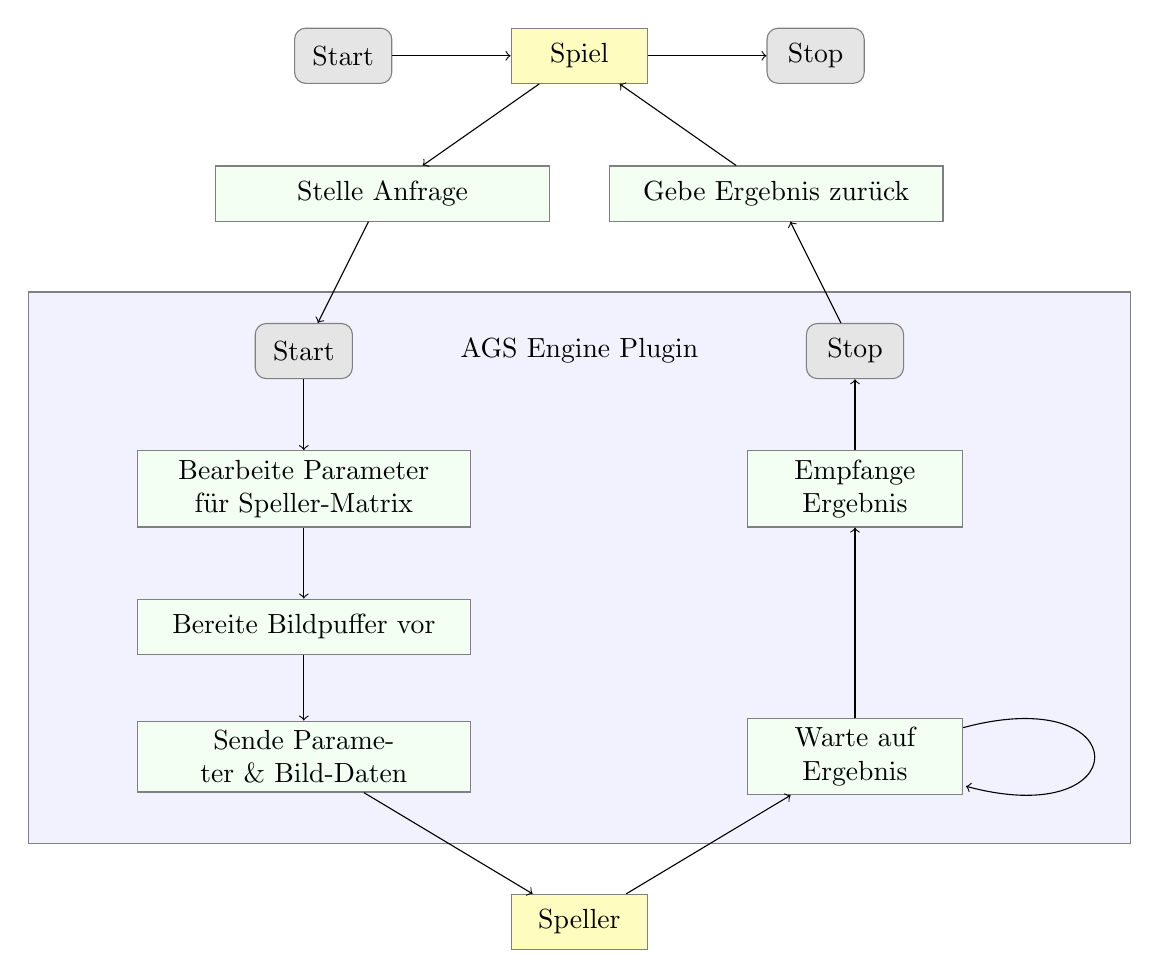
\begin{tikzpicture}[scale=1.0,
rectStart/.style={rectangle, draw=black!50, fill=black!10, minimum width=5mm, minimum height=7mm, text width=10mm, align=center, rounded corners},
rectStart2/.style={rectangle, draw=black!50, fill=black!10, minimum width=5mm, minimum height=7mm, text width=20mm, align=center, rounded corners},
rectDoWork/.style={rectangle, draw=black!50, fill=green!5, minimum width=5mm, minimum height=7mm, text width=40mm, align=center},
rectDoWork2/.style={rectangle, draw=black!50, fill=green!5, minimum width=5mm, minimum height=7mm, text width=25mm, align=center},
rectDoWorkSmall/.style={rectangle, draw=black!50, fill=green!5, minimum width=5mm, minimum height=7mm, text width=15mm, align=center},
rectMisc/.style={rectangle, draw=black!50, fill=yellow!25, minimum width=5mm, minimum height=7mm, text width=15mm, align=center},
rectPlugin/.style={rectangle, draw=black!50, fill=blue!5, minimum width=140mm, minimum height=70mm, text width=110mm, align=center},
rectText/.style={minimum width=5mm, minimum height=10mm, text width=40mm, align=center}]


\node[rectStart] (start) at (-3, 3) {Start};
\node[rectMisc] (spiel) at (0, 3) {Spiel};
\node[rectStart] (stop) at (3, 3) {Stop};

\node[rectDoWork] (request) at (-2.5, 1.25) {Stelle Anfrage};
\node[rectDoWork] (result) at (2.5, 1.25) {Gebe Ergebnis zurück};

\node[rectPlugin] (plugin) at (0, -3.5) {};
\node[rectText] (pluginText) at (0, -0.75) {AGS Engine Plugin};

\node[rectStart] (startPlugin) at (-3.5, -0.75) {Start};
\node[rectStart] (stopPlugin) at (3.5, -0.75) {Stop};


\node[rectMisc] (speller) at (0, -8) {Speller};

\node[rectDoWork] (params) at (-3.5, -2.5) {Bearbeite Parameter für Speller-Matrix};
\node[rectDoWork] (image) at (-3.5, -4.25) {Bereite Bildpuffer vor};
\node[rectDoWork] (send) at (-3.5, -5.9) {Sende Parameter \& Bild-Daten};
\node[rectDoWork2] (waitresult) at (3.5, -5.9) {Warte auf Ergebnis};
\node[rectDoWork2] (recvresult) at (3.5, -2.5) {Empfange Ergebnis};


 \path[->] 	(start) 				edge 					node {} (spiel)
			(spiel) 				edge 					node {} (request)
			(result) 				edge 					node {} (spiel)
			(request) 				edge 					node {} (startPlugin)
			(stopPlugin) 			edge 					node {} (result)
			(startPlugin) 			edge 					node {} (params)
			(params) 				edge 					node {} (image)
			(image) 				edge 					node {} (send)
			(send) 					edge 					node {} (speller)		
			(speller) 				edge 					node {} (waitresult)
			(waitresult) 			edge 		[loop right]node {} (waitresult)
			(waitresult) 			edge 					node {} (recvresult)			
			(recvresult) 			edge 					node {} (stopPlugin)			
			(spiel) 				edge 					node {} (stop);


\end{tikzpicture}
\caption{Der Ablauf einer Anfrage des Spiels an das AGS Engine Plugin und die damit verbundenen Schritt bis zur Rückgabe des Ergebnisses}
\label{pluginPlan}
\end{center}
\end{figure}

\pagebreak

Beim Starten des Spiels wird zunächst eine TCP/IP-Verbindung zum AGS-P300-Speller aufgebaut.
Da das Plugin den Clienten einer Client-Server-Kommunikation darstellt ist es notwendig, dass der Speller bereits gestartet ist und auf die Verbindung des Plugins wartet.
Von diesem Zeitpunkt an ist das Plugin bereit, Anfragen des Spiels weiterzuleiten.
Eine Anfrage erfolgt durch Aufrufen einer Methode innerhalb des Spiels.
Diese Methode erwartet die Parameter zum Aufspannen der Speller-Matrix.
Das Plugin wird die Daten zunächst für den Sende-Vorgang vorbereiten und anschließend die Bild-Daten des Spiels von der Engine abfragen.
An dieser Stelle ist es nötig die Farbkanal-Repräsentation der Bild-Daten in \acs{RGBA} umzuwandeln, da der aktuelle Spielausschnitt von der Engine hingegen in \acs{BGRA} bereitstellt wird.
Die vorbereiteten Daten werden anschließend an den Speller gesendet.
Das Plugin wartet daraufhin auf das Ergebnis, welches dem ausgewählten Matrix-Element entspricht.
Nach weiterreichen des Ergebnisses wartet das Plugin auf eine erneute Anfrage, um den Vorgang zu wiederholen.\\








\pagebreak
\section{Erstellung des Point\&Click Test-Spiels}

Nach der Entwicklung des Spellers und des Plugins ist es notwendig diese zu testen.
Daher wird nachfolgend ein kleines Test-Spiel entwickelt, um die entwickelten Funktionen zu überprüfen.
Wie im Konzept geschrieben wird es sich optisch an "`The Secret of Monkey Island "' anlehnen.\\

Zur Entwicklung des Spiels wird das Adventure Game Studio in der Version 3.3.0 verwendet.
Weiterhin wird das AGS Engine Plugin im Spiel referenziert und geladen, sodass dessen Funktionen zur Verfügung stehen.\\

Das Spiel-Szenario verwendet eine Strandkulisse, die in Abbildung\footnote[1]{Bild-Quelle: \cite{JM2014}} \ref{strand1} zu sehen ist.
Sie wird im Hintergrund des Spiels dargestellt und je eine Hälfte bildet einen "`Raum"' bzw. eine Szene ab.\\

\begin{figure}[ht]
\centering
\includegraphics[scale=0.88]{images/MI_beach.png}
\caption{Die Strandkulisse des Test-Spiels}
\label{strand1}
\end{figure}

Während des Spiels soll eine Spielfigur über einen Strand bewegt werden, um Gegenstände auf dem Strand aufzuheben oder die Szenen zu wechseln.
Die Steuerung erfolgt hierbei über zwei Eingabe-Ermittlungen des Spellers.
Die erste ermittelt den auszuführenden Befehl, die zweite das Ziel des Befehls.
Bei der Befehlsauswahl kann es bei einer falschen Auswahl dazu kommen, dass ein Matrix-Element ausgewählt wird, dem kein Befehl zugeordnet ist. 
In einem solchen Fall wird die Befehlsauswahl wiederholt.\\

\pagebreak

Die notwendige Mindestgröße der Speller-Matrix sorgt bei der Befehlsauswahl dafür, 
dass die einzelnen Befehle mit mehreren Zeilen überlagert werden, 
um so dem Oddball-Paradigma zu entsprechen (siehe Abbildung \ref{Befehlsauswahl}).
Dies führt dazu, dass ein Befehl von mehreren Matrix-Elementen abgedeckt wird und ein Befehl demzufolge bei mehreren Speller-Ergenissen ausgewählt werden kann.\\

\begin{figure}[ht]
\centering
\includegraphics[scale=0.5]{images/Befehlsauswahl.png}
\caption{Die Befehlsauswahl des Test-Spiels}
\label{Befehlsauswahl}
\end{figure}

Bei der Zielauswahl gilt es ebenfalls eine Mindestgröße einzuhalten.
Allerdings ist es ebenfalls sinnvoll die Größe der Speller-Matrix zu begrenzen, da zu kleine Matrix-Elemente deren Fokussierung erschweren.
Zusätzlich würde dies einem Benutzer erhöhte Konzentration abverlangen und birgt die Gefahr, dass Ergebnisse negativ beeinflusst werden.
In Abbildung \ref{Zielauswahl} wird die Speller-Matrix der Zielauswahl dargestellt, die den gesamten begehbaren Bereich des Spiels umfasst.
Die drei in dieser Szene einzusammelnden Objekte sind ebenfalls zu sehen.\\


\begin{figure}[ht]
\centering
\includegraphics[scale=0.5]{images/Zielauswahl.png}
\caption{Die Zielauswahl des Test-Spiels}
\label{Zielauswahl}
\end{figure}

Mit Hinblick auf die Tests wurde das Spiel mit zwei Szenen und insgesamt sechs Objekten ausgestattet.
Es gibt drei Befehle "`Gehen"', "`Aufheben"' und "`Beenden"'.\\
Mit "`Gehen"' bewegt sich die Spielfigur an die ausgewählte Position. 
Um die Szene zu wechseln ist es beispielsweise erforderlich an den Rand der aktuellen Szene zu gehen.
Mit "`Aufheben"' bewegt sich die Spielfigur nur dann zum ausgewählten Feld, wenn sich dort ein Gegenstand befindet und hebt diesen dann auf, andernfalls würde eine Sprechblase erscheinen, dass es dort nichts aufzuheben gibt. \\
Der "`Beenden"'-Befehl beendet das Spiel, sofern dieser zwei mal in Folge ausgewählt wurde, andernfalls könnte das Spiel versehentlich bei einer falschen Eingabe beendet werden.\\

Das Aufheben eines Objekts und das Wechseln der Szene ist jeweils mit zwei Eingaben verbunden.
Daraus ergibt sich, dass das Spiel in insgesamt 14 Eingabe-Ermittlungen beendet ist, sofern eine Genauigkeit von 100\% vorliegt.


















